\documentclass[11pt]{article}

\usepackage[letterpaper,margin=0.72in]{geometry}
\usepackage{amsmath}
\usepackage{array}
\usepackage{booktabs}
\usepackage{caption}
\usepackage{xcolor}
\usepackage{fancyhdr}
\usepackage{graphicx}
\usepackage{hyperref}
\usepackage[nopatch=footnote]{microtype}
\usepackage{enumitem}
\usepackage{setspace}
\usepackage{tabularx}
\usepackage{xurl}

\definecolor{reportblue}{HTML}{24557A}
\definecolor{reportred}{HTML}{B34B58}
\hypersetup{
  colorlinks=true,
  linkcolor=reportblue,
  urlcolor=reportblue,
  citecolor=reportblue,
  pdfauthor={Chengzong Liu},
  pdftitle={Learning Route Value to Improve a Ticket to Ride: Europe Optimizer}
}
\pagestyle{fancy}
\fancyhf{}
\fancyhead[L]{\small CSE 163 Final Project}
\fancyhead[R]{\small Ticket to Ride: Europe}
\fancyfoot[C]{\thepage}
\renewcommand{\headrulewidth}{0.4pt}
\setstretch{1.12}
\setlength{\parindent}{0pt}
\setlength{\parskip}{4pt}
\setlist{leftmargin=*,itemsep=2pt,topsep=3pt}
\captionsetup{font=normalsize,labelfont=bf,skip=3pt}
\newcommand{\code}[1]{\texttt{#1}}

\begin{document}

\thispagestyle{fancy}
\section*{1. Title and Author(s)}

\begin{center}
{\LARGE\bfseries Learning Route Value to Improve a\\[3pt]
Ticket to Ride: Europe Optimizer}\par
\vspace{0.28in}
{\large Chengzong Liu}\par
CSE 163 A $\mid$ Summer 2026 $\mid$ Final Project, Part 3\par
\vspace{0.15in}
\textbf{Public code repository:}\par
\href{https://github.com/liuchengzong291817-ui/cse163-ticket-to-ride}
{github.com/liuchengzong291817-ui/cse163-ticket-to-ride}
\end{center}

\section*{2. Summary of Questions and Results}

\begin{enumerate}[label=\textbf{RQ\arabic*.}]
  \item \textbf{Which structural features make a destination ticket
  efficient?} Printed points almost reproduce minimum train cost
  ($r=0.995$), and 39 of 46 tickets have exact equality. Points per minimum
  train stay between 0.800 and 1.125. Redundancy, detour cost, and cut edges
  therefore distinguish fragility more than printed value.

  \item \textbf{How accurately can map-derived features predict printed
  ticket points?} Ridge was best: repeated outer-fold MAE was
  $0.378\pm0.077$ points and $R^2=0.975\pm0.025$; its averaged out-of-fold
  (OOF) MAE was 0.361 and $R^2=0.987$. The mean baseline's MAE was
  $3.413\pm1.002$, so the model learned strong out-of-sample structure.

  \item \textbf{Does learned route value improve the 45-train optimizer?}
  No under the predeclared primary criterion. Across 250 matched 12-ticket
  pools, median total points per train fell from 3.000 to 2.955 and median
  printed ticket points fell from 67 to 66. Median worst-edge retention rose
  from 0.703 to 0.744, revealing a small robustness--efficiency tradeoff, but
  not an overall improvement. Every plan respected the 45-train limit.
\end{enumerate}

\vfill
\textit{All numerical claims in this report are regenerated by
\code{python analysis.py} from the three CSV files in the public repository.}

\newpage
\section*{3. Motivation}

Ticket to Ride is a graph-planning problem under a scarce train budget. A
shortest path can connect a ticket cheaply, yet it may depend on a contested
edge, lack a useful alternate route, or contribute little to other accepted
tickets. My earlier single-player heuristic encoded those tradeoffs with
fixed weights. This project asks whether evidence learned from the Europe map
can replace part of that hand-designed judgment.

The analysis has two practical goals. First, it explains how the published
ticket deck rewards distance, efficiency, and redundancy. Second, it tests a
data-driven modification under exactly matched planning situations rather
than showing one favorable example. A negative optimizer result is useful:
it identifies when a simple, observable rule is already difficult to beat.

\section*{4. Dataset}

The project uses the three public CSV files in Leon Simon's \textit{Data \&
Analysis of Ticket to Ride: Europe} repository [1]. The copies in this
project are preserved as raw inputs. Table~\ref{tab:data} reports their actual
dimensions after loading. The combined table has one row per destination
ticket and attaches graph and geographic features to its two endpoints.

\begin{table}[h]
\centering
\caption{Dataset dimensions and missingness after validation.}
\label{tab:data}
\begin{tabular}{lrrr}
\toprule
Dataset & Rows & Columns & Missing values \\
\midrule
\code{cities.csv} & 47 & 3 & 0 \\
\code{routes.csv} & 90 & 6 & 0 \\
\code{destinations.csv} & 46 & 3 & 0 \\
Combined ticket feature table & 46 & 20 & 0 \\
\bottomrule
\end{tabular}
\end{table}

\code{cities.csv} supplies city names, longitude, and latitude.
\code{routes.csv} supplies adjacent endpoints, carriage cost, color status,
tunnel status, and locomotive requirement. \code{destinations.csv} supplies
ticket endpoints and the response variable, printed \code{Points}. Validation
found 47 unique city names, positive route costs and ticket points, no missing
endpoints, and no duplicated unordered city pair. Although the proposal
planned to preserve parallel routes, this particular extracted dataset has
none; the final method therefore treats each unordered pair as one edge.

The unit of analysis for RQ1 and RQ2 is one of the 46 destination tickets.
RQ3 samples matched pools of those tickets and evaluates the shared network
that can be constructed with at most 45 trains, the official per-player
supply [2].

\newpage
\section*{5. Method: Validation and Graph Features}

\textbf{Graph construction.} After trimming city strings, the program checks
required columns, missing values, positive quantities, unique cities,
unordered-route duplication, and endpoint membership. It then creates an
undirected adjacency list weighted by route carriage count. A custom
Dijkstra implementation returns minimum cost, one deterministic minimum
path, and the number of equally short paths. Removing one edge at a time and
rerunning Dijkstra supplies the detour and cut-edge measures.

\textbf{Geographic and structural measurements.} For endpoints with
longitude $\lambda$ and latitude $\phi$, straight-line distance is the
haversine distance
\[
d=2R\arcsin\!\left(\sqrt{\sin^2\!\left(\frac{\Delta\phi}{2}\right)+
\cos\phi_1\cos\phi_2\sin^2\!\left(\frac{\Delta\lambda}{2}\right)}\right),
\quad R=6371\text{ km}.
\]
Each ticket also receives minimum trains, points per minimum train, equal
minimum-path count, largest finite edge-removal detour, a cut-edge indicator,
mean route length, intermediate-city count, and tunnel/ferry fractions.

\textbf{Overlap measure.} The descriptive high-value overlap feature counts
how often each representative minimum-path edge occurs among tickets at or
above the 75th point percentile. A ticket's own contribution is removed
before averaging across its edges. This feature helps describe reuse in RQ1,
but it is derived from \code{Points}; it is excluded from every RQ2 model and
from the learned penalty. \code{points\_per\_train} is excluded for the same
reason.

\textbf{Scoring.} Route points use the official Europe table [2]: lengths 1,
2, 3, 4, 6, and 8 score 1, 2, 4, 7, 15, and 21 points. The final analysis is
Europe-specific. The earlier USA-map simulation was used only as conceptual
background and is neither submitted as an analysis module nor used to
produce these results.

\textbf{Interpretation boundary.} Path choice is deterministic when multiple
minimum paths tie, so path-specific detour and overlap describe one
representative solution. Equal-path count separately records the tie. These
are associations on a fixed game board, not causal effects or observations
of human play.

\newpage
\section*{5. Method: Machine Learning}

The response is printed ticket points. The nine permitted predictors are
minimum trains, straight-line distance, equal minimum-path count, maximum
detour, cut-edge indicator, mean edge length, intermediate cities, tunnel
fraction, and ferry fraction. Neither the response nor any column calculated
from it enters the predictor matrix.

\textbf{Models.} A fold-trained mean baseline predicts the training mean.
Ridge regression standardizes predictors inside its pipeline and
tests $\alpha\in\{0.01,0.1,1,10,100\}$. The random forest tests 100 or 300
trees, depth unrestricted/3/5, and minimum leaf size 1/2/4. These models
provide a simple reference, an interpretable regularized linear model, and a
nonlinear alternative.

\textbf{Nested repeated evaluation.} The outer evaluation is five-fold
cross-validation repeated five times with seed 163, producing 25 matched
outer folds [3]. Within each outer training set, a shuffled four-fold grid
search selects hyperparameters by negative MAE. Scaling, tuning, and fitting
therefore occur without the outer test tickets. Every ticket receives five
held-out predictions; their mean is its OOF value. Models are compared by
outer-fold MAE and $R^2$, reported as mean $\pm$ sample standard deviation,
plus metrics on the averaged OOF predictions.

\textbf{Interpretation.} Ridge coefficients are recorded after training-fold
standardization. For each tuned random forest, each feature is shuffled ten
times only in that outer test fold; the increase in MAE is then averaged over
folds. Held-out permutation importance estimates a model's dependence on a
feature for generalization, not the feature's causal effect [4].

The same folds and seed are used for every model. Negative fold $R^2$ is
possible for a weak model because each test fold contains only nine or ten
tickets; MAE is the primary predictive metric. The optimizer uses only the
lowest-OOF-MAE model selected by this procedure. (Here ``OOF'' means a ticket
was never in the training data for its own prediction.)

\newpage
\section*{5. Method: Optimizer and Matched Evaluation}

Every trial samples 12 tickets without replacement and treats them as an
already accepted planning pool. The original and revised methods receive the
identical pool, route map, tie-breaking rule, and 45-train budget. This is a
controlled network-planning benchmark, not a simulation of drawing cards,
opponents, or turns.

Let $d_j$ be printed points, $C_j$ the marginal trains for the least-cost path
given the existing network, and $G_j$ the route points on newly required
edges. The original heuristic ranks each feasible ticket by
\[
V_j=d_j+G_j-3C_j.
\]
It greedily adds the best feasible ticket and reuses already selected edges
at zero marginal cost. Because tickets are treated as accepted, negative
$V_j$ affects order but does not cancel an obligation; selection continues
until no remaining path fits.

For the revised method, Ridge OOF prediction $\hat d_j$ adds only its
estimated premium above standalone minimum cost $L_j$:
\[
\widetilde d_j=d_j+(\hat d_j-L_j).
\]
The score then subtracts
$0.20\widetilde d_j\bar b_j$, where $\bar b_j\in[0,1]$ is mean normalized
usage of that path's edges by the current ticket pool. The 20\% maximum
dependence penalty was fixed before comparing outcomes and was not tuned to
make the revised method win.

There are 250 matched pools from seed 163. Primary success requires higher
median total points per train, no plan above 45 trains, and no material
(greater than two percentage-point) decline in mean or worst blocked-edge
retention. Total points equal printed points plus official route points.
Robustness removes each of the five edges most frequently used by all 46
representative ticket paths. Post-hoc tests allow no repair; adaptive tests
rerun the planner with that edge unavailable.

\newpage
\section*{6. Exploratory Data Analysis}

Figure~\ref{fig:eda} connects ticket reward, minimum resource cost, and
fragility. Printed points average 9.63 (SD 4.66), while minimum trains average
9.59 (SD 4.52). Their Pearson correlation is 0.995. Ticket efficiency averages
1.00 point per minimum train (SD 0.04), despite maximum finite detours ranging
from 0 to 19 trains.

\begin{figure}[h]
\centering
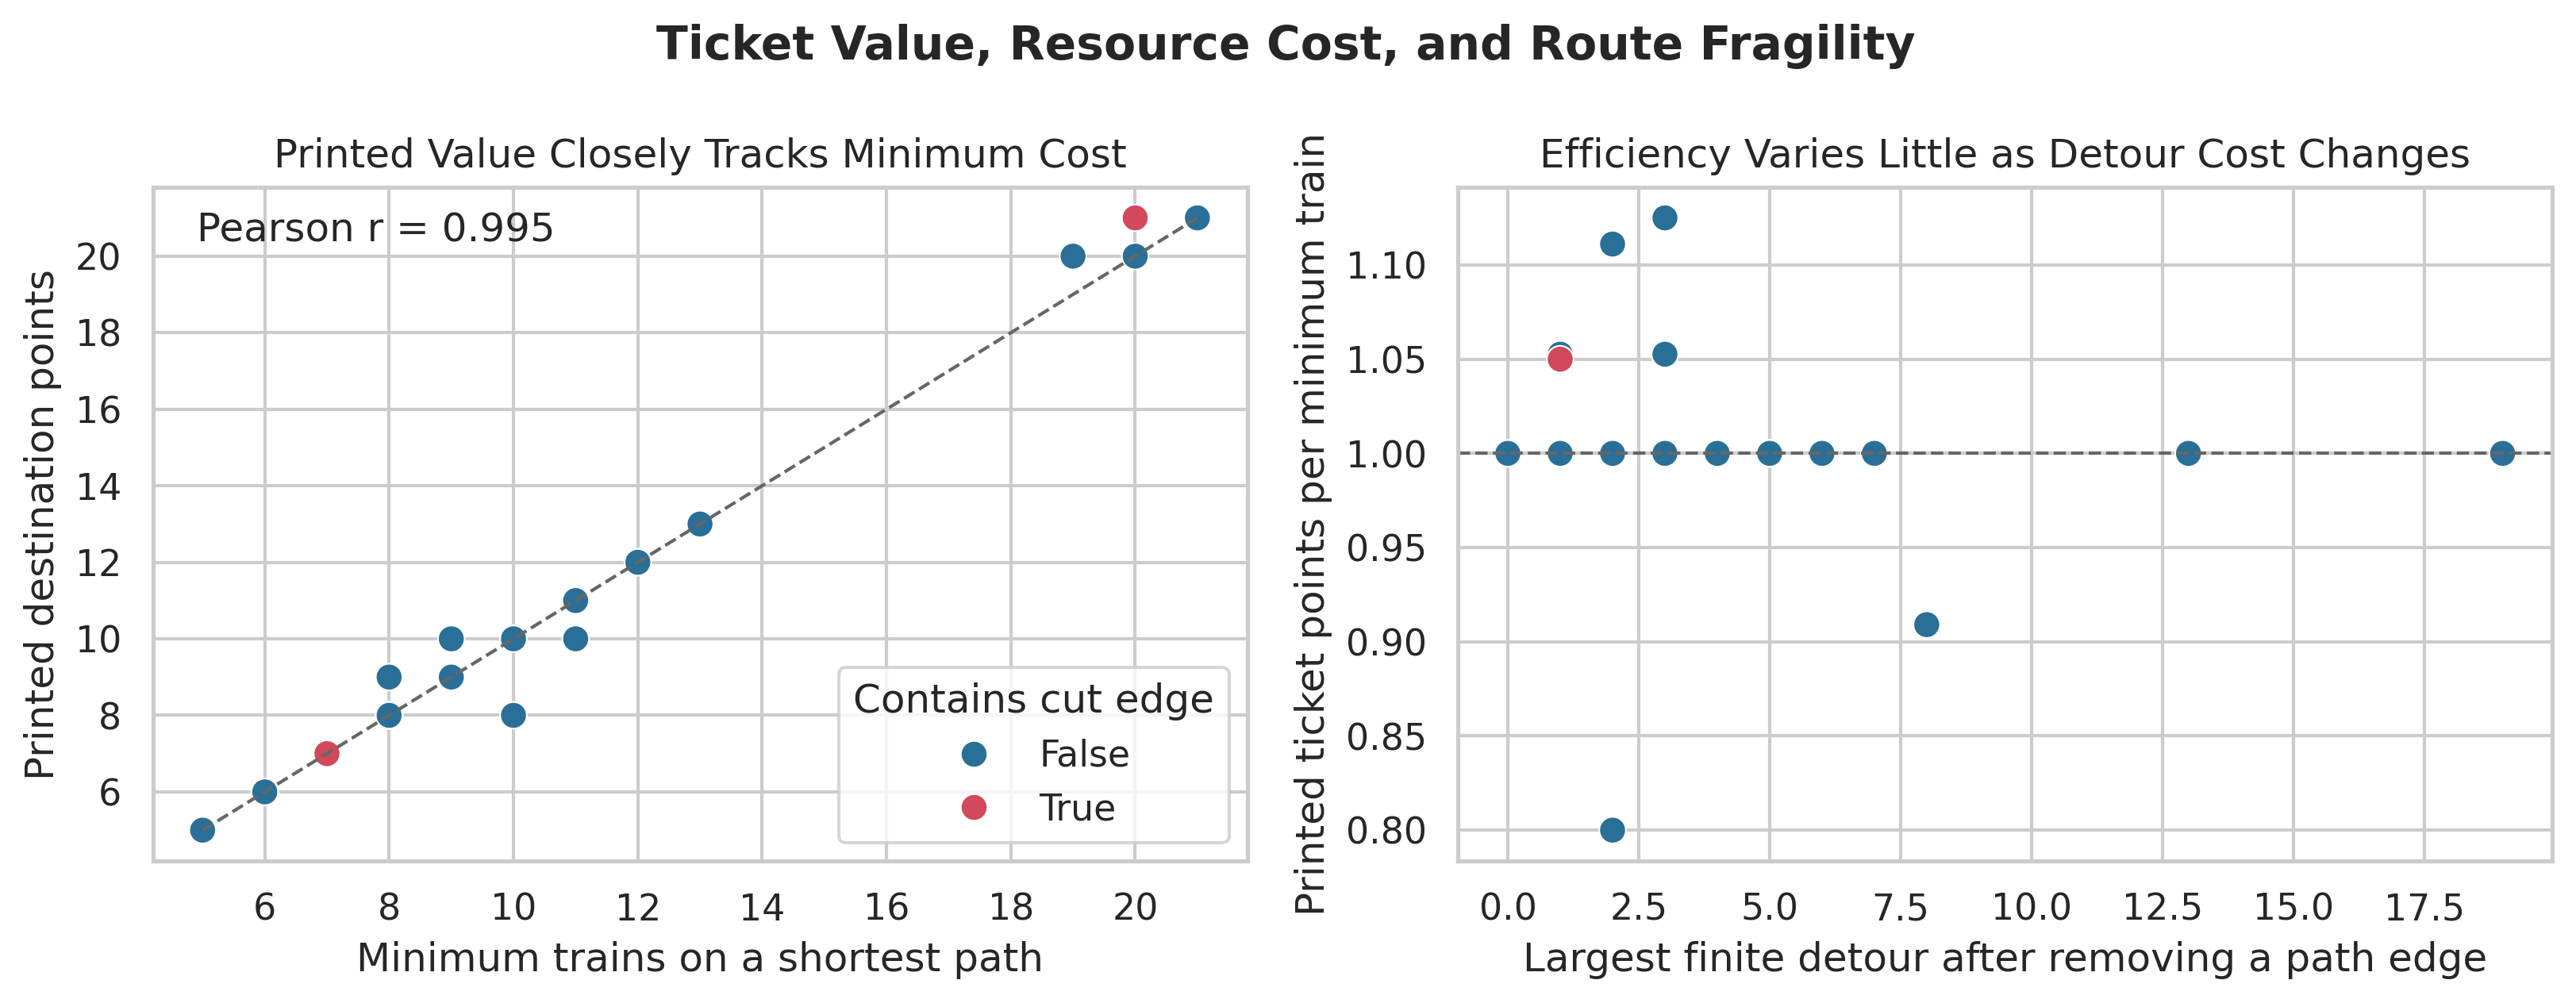
\includegraphics[width=0.98\textwidth]{../figures/eda_relationships.png}
\caption{\textbf{Ticket value, minimum cost, and route fragility.} Left:
printed points nearly follow the one-to-one dashed line; red marks the two
tickets whose representative minimum paths contain a cut edge. Right:
efficiency occupies a narrow band even as finite detour cost changes. The
plots were generated from \code{feature\_table.csv} with seaborn.}
\label{fig:eda}
\end{figure}

The combined table has no missing values. Thirty-five tickets have one
minimum path, ten have two, and one has three. Only Edinburgh--Paris and
Edinburgh--Athina contain a cut edge on the selected minimum path. These
observations motivate (1) a strong minimum-cost predictor for RQ2 and (2) a
separate robustness objective for RQ3. The EDA did not justify using
target-derived efficiency or high-value overlap as model predictors, so both
remain descriptive only.

\newpage
\section*{7. Results: RQ1 -- Efficient and Robust Tickets}

Table~\ref{tab:rq1} summarizes the main structural results. The strongest
finding is near identity between printed value and minimum cost: 39 of 46
tickets lie exactly on the line in Figure~\ref{fig:eda}. Bruxelles--Danzic is
the most efficient ticket (9 points for 8 minimum trains, 1.125), while
Palermo--Constantinople is least efficient (8 for 10, 0.800).

\begin{table}[h]
\centering
\caption{Principal RQ1 summaries from all 46 destination tickets.}
\label{tab:rq1}
\begin{tabularx}{\textwidth}{Xrrrrr}
\toprule
Variable & Mean & SD & Minimum & Median & Maximum \\
\midrule
Printed points & 9.63 & 4.66 & 5.00 & 8.00 & 21.00 \\
Minimum trains & 9.59 & 4.52 & 5.00 & 8.00 & 21.00 \\
Ticket points/minimum train & 1.00 & 0.04 & 0.80 & 1.00 & 1.125 \\
Straight-line distance (km) & 1329.38 & 628.72 & 556.28 & 1159.75 & 3080.39 \\
Equal minimum paths & 1.26 & 0.49 & 1.00 & 1.00 & 3.00 \\
Maximum finite detour & 3.30 & 3.27 & 0.00 & 3.00 & 19.00 \\
High-value edge overlap & 1.03 & 0.74 & 0.00 & 1.00 & 3.00 \\
\bottomrule
\end{tabularx}
\end{table}

Frankfurt--Khobenhaven has the maximum observed detour: removing a selected
path edge adds 19 trains to the best remaining route. London--Berlin has the
maximum descriptive high-value overlap of 3. These examples show why a
ticket can have ordinary printed efficiency while differing sharply in
backup cost or network reuse.

\textbf{Answer to RQ1.} Minimum train cost explains almost all printed value;
geographic scale and intermediate-city count provide secondary scale
information. Redundancy and edge-removal measures supply a distinct
strategic dimension. They identify fragility, but the small number of cut
cases and representative-path convention prevent a claim that they cause
better or worse gameplay outcomes.

\newpage
\section*{7. Results: RQ2 -- Predictive Accuracy}

Table~\ref{tab:models} and Figure~\ref{fig:model} show that both trained models
greatly outperform the fold-trained mean. Ridge has the lowest MAE. Its most
common selected $\alpha$ is 0.01 (13 of 25 folds), followed by 0.1 (10 folds)
and 1 (2 folds). Random-forest choices vary, which is consistent with only 46
observations.

\begin{table}[h]
\centering
\caption{Leakage-free nested/repeated cross-validation results.}
\label{tab:models}
\begin{tabular}{lrrrrrr}
\toprule
Model & Fold MAE & SD & Fold $R^2$ & SD & OOF MAE & OOF $R^2$ \\
\midrule
Ridge & 0.378 & 0.077 & 0.975 & 0.025 & 0.361 & 0.987 \\
Random forest & 0.467 & 0.309 & 0.955 & 0.065 & 0.428 & 0.980 \\
Mean baseline & 3.413 & 1.002 & $-0.294$ & 0.450 & 3.403 & $-0.047$ \\
\bottomrule
\end{tabular}
\end{table}

\begin{figure}[h]
\centering
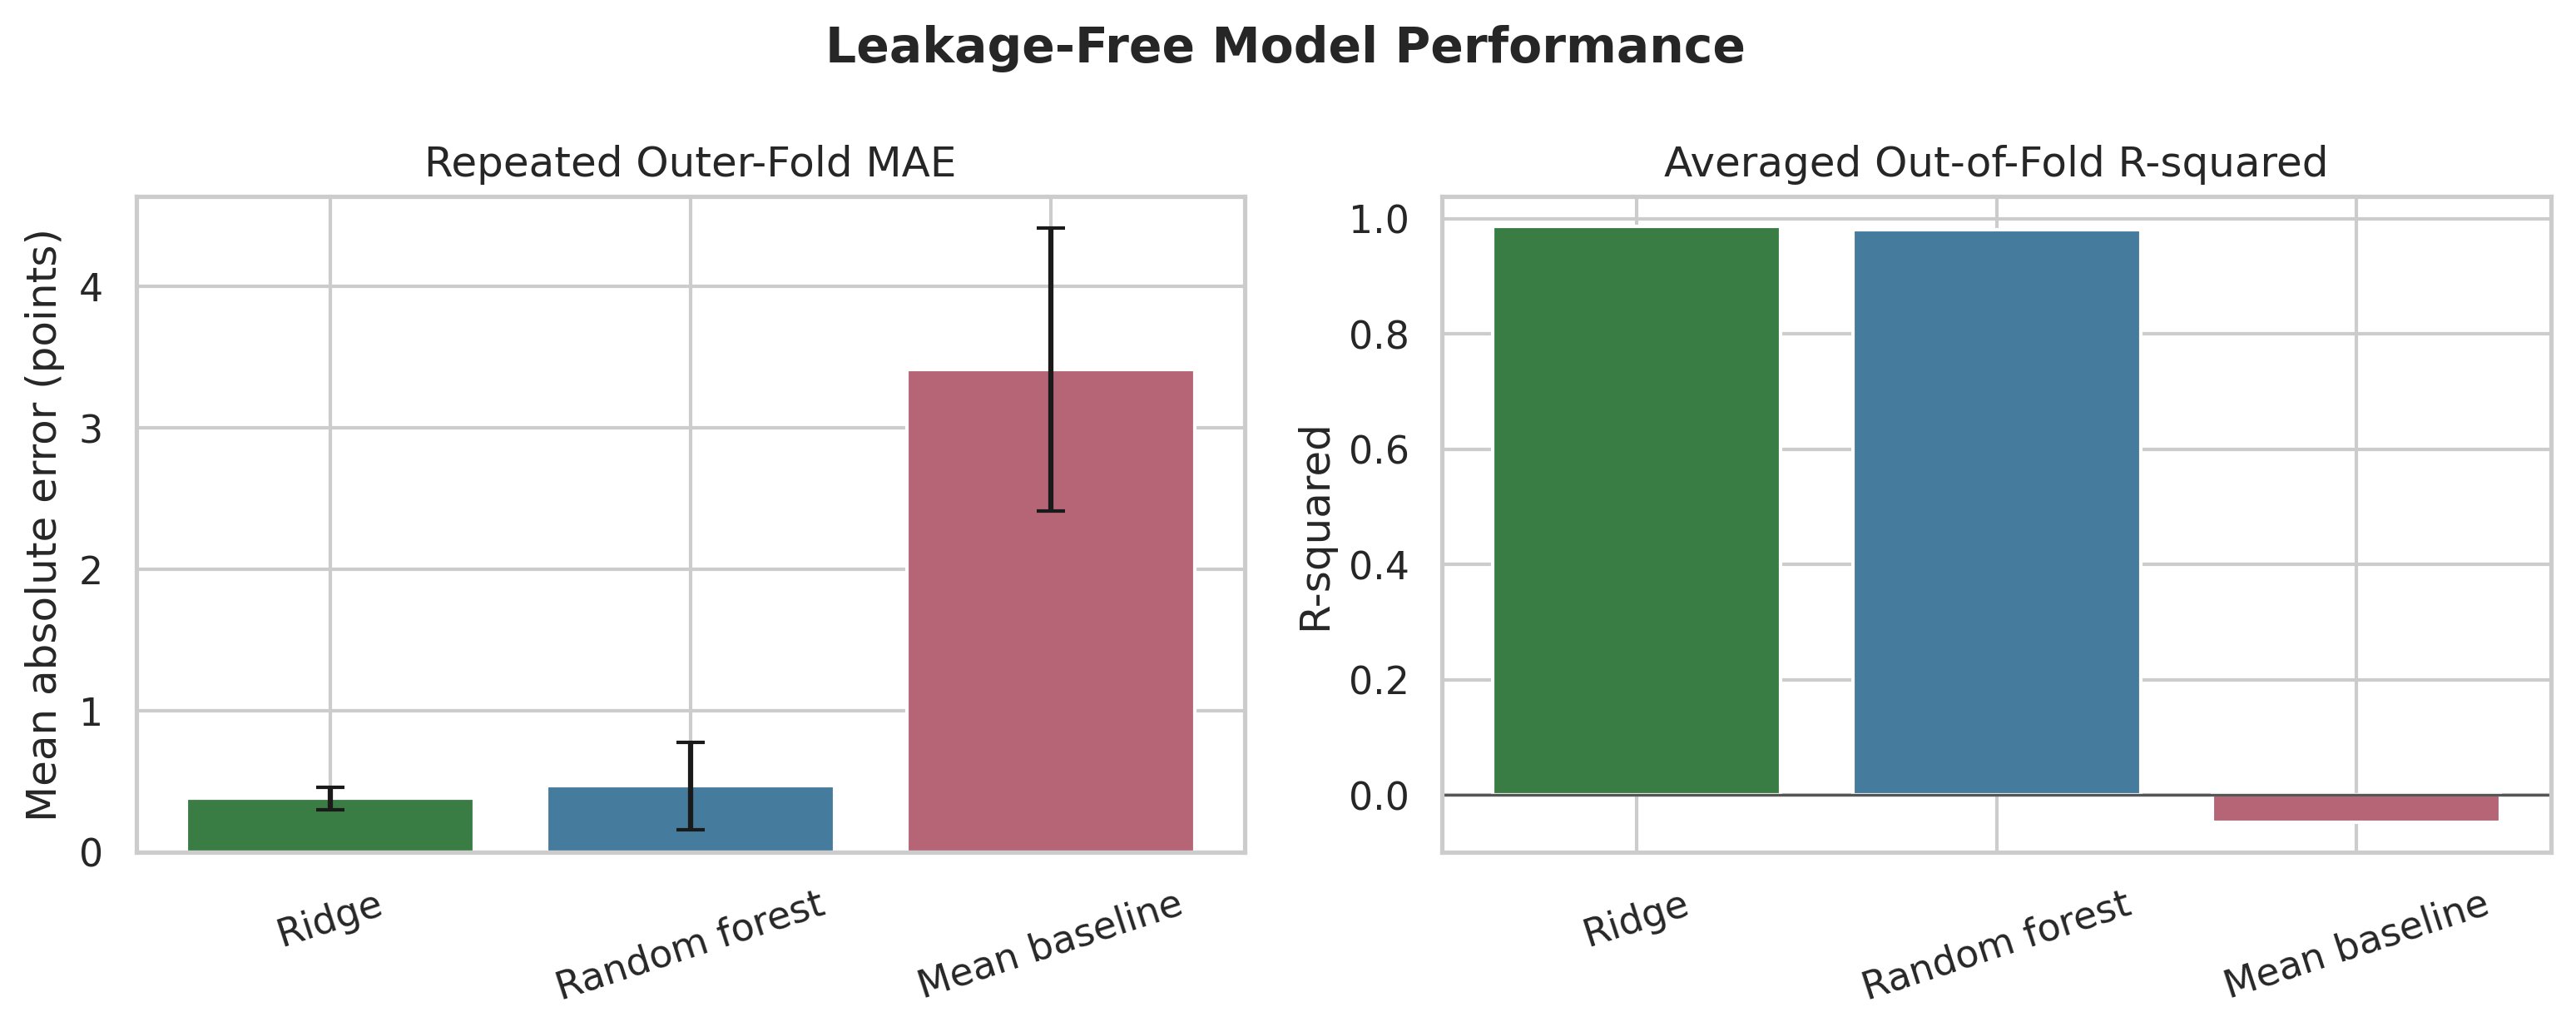
\includegraphics[width=0.91\textwidth]{../figures/model_comparison.png}
\caption{\textbf{Model performance on unseen tickets.} Error bars are the
sample SD across 25 outer folds; the right panel evaluates one averaged OOF
prediction per ticket. All preprocessing and tuning occur inside training
folds.}
\label{fig:model}
\end{figure}

Ridge reduces mean outer-fold MAE by 3.035 points, or 88.9\%, relative to the
mean baseline. The result easily meets the proposal's requirement that the
best model improve on that baseline. However, this is not evidence that an
arbitrary board can be predicted: the model learns the specific Europe deck,
where printed points almost encode minimum path length.

\newpage
\section*{7. Results: RQ2 -- Held-Out Predictions and Interpretation}

Figure~\ref{fig:oof} shows that every Ridge point is close to the identity
line. The largest visible residuals occur among tickets where printed points
depart from the near one-for-one cost rule; this is exactly where a learned
premium could change an optimizer's ordering.

\begin{figure}[h]
\centering
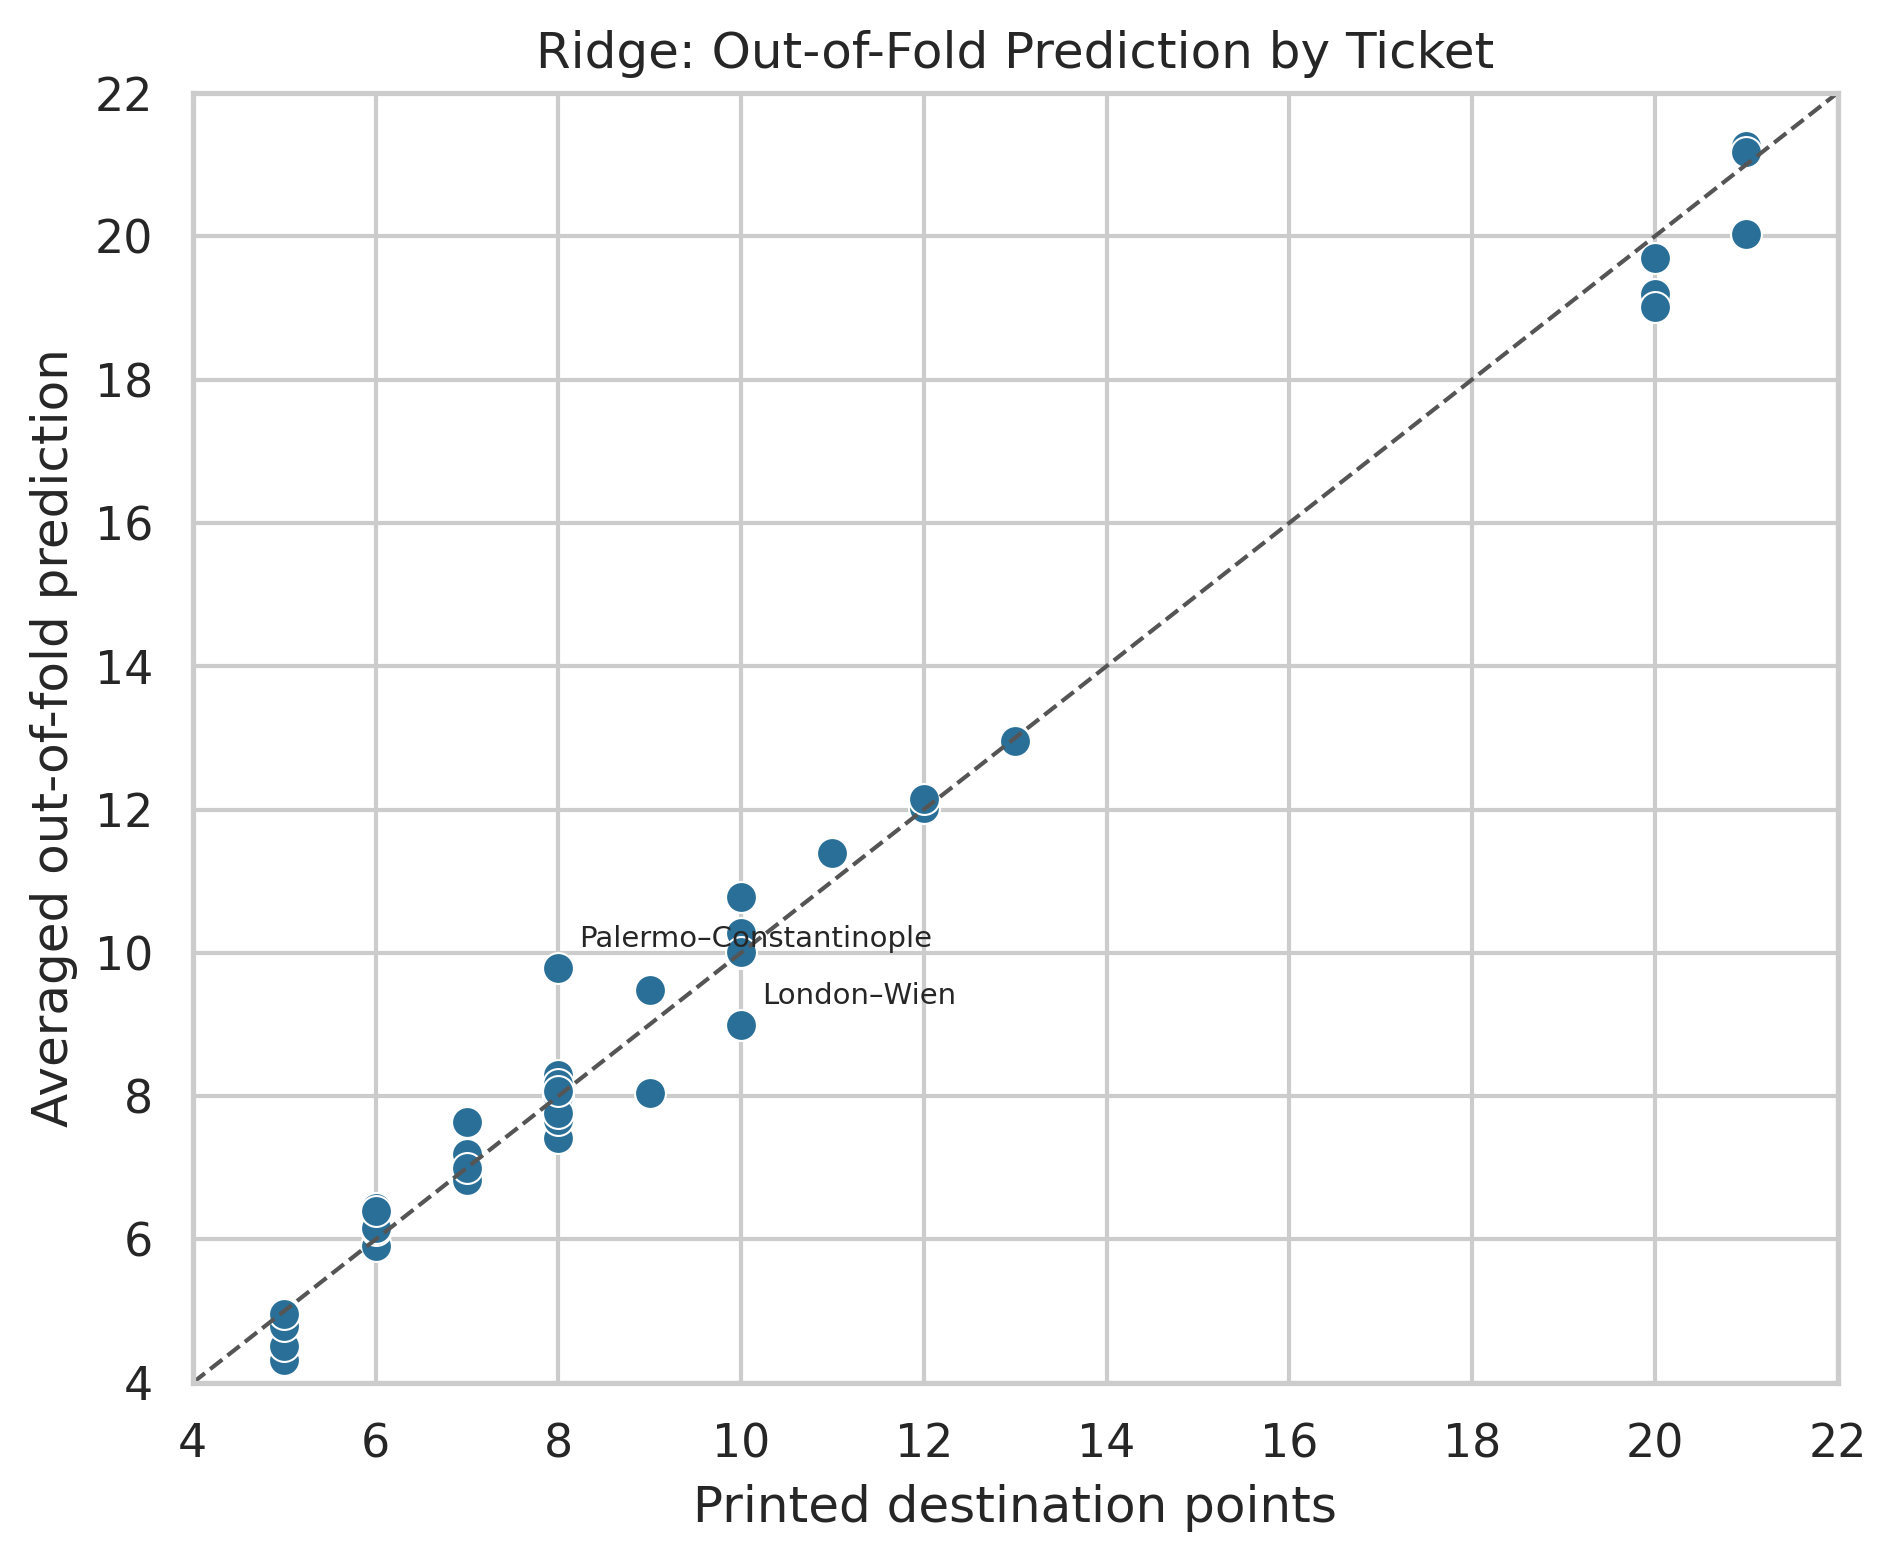
\includegraphics[width=0.56\textwidth]{../figures/oof_predictions.png}
\caption{\textbf{Printed versus Ridge OOF points.} Each coordinate is averaged
over five models that did not train on that ticket. The dashed line denotes
perfect prediction; the three largest absolute residuals are labeled.}
\label{fig:oof}
\end{figure}

\begin{figure}[h]
\centering
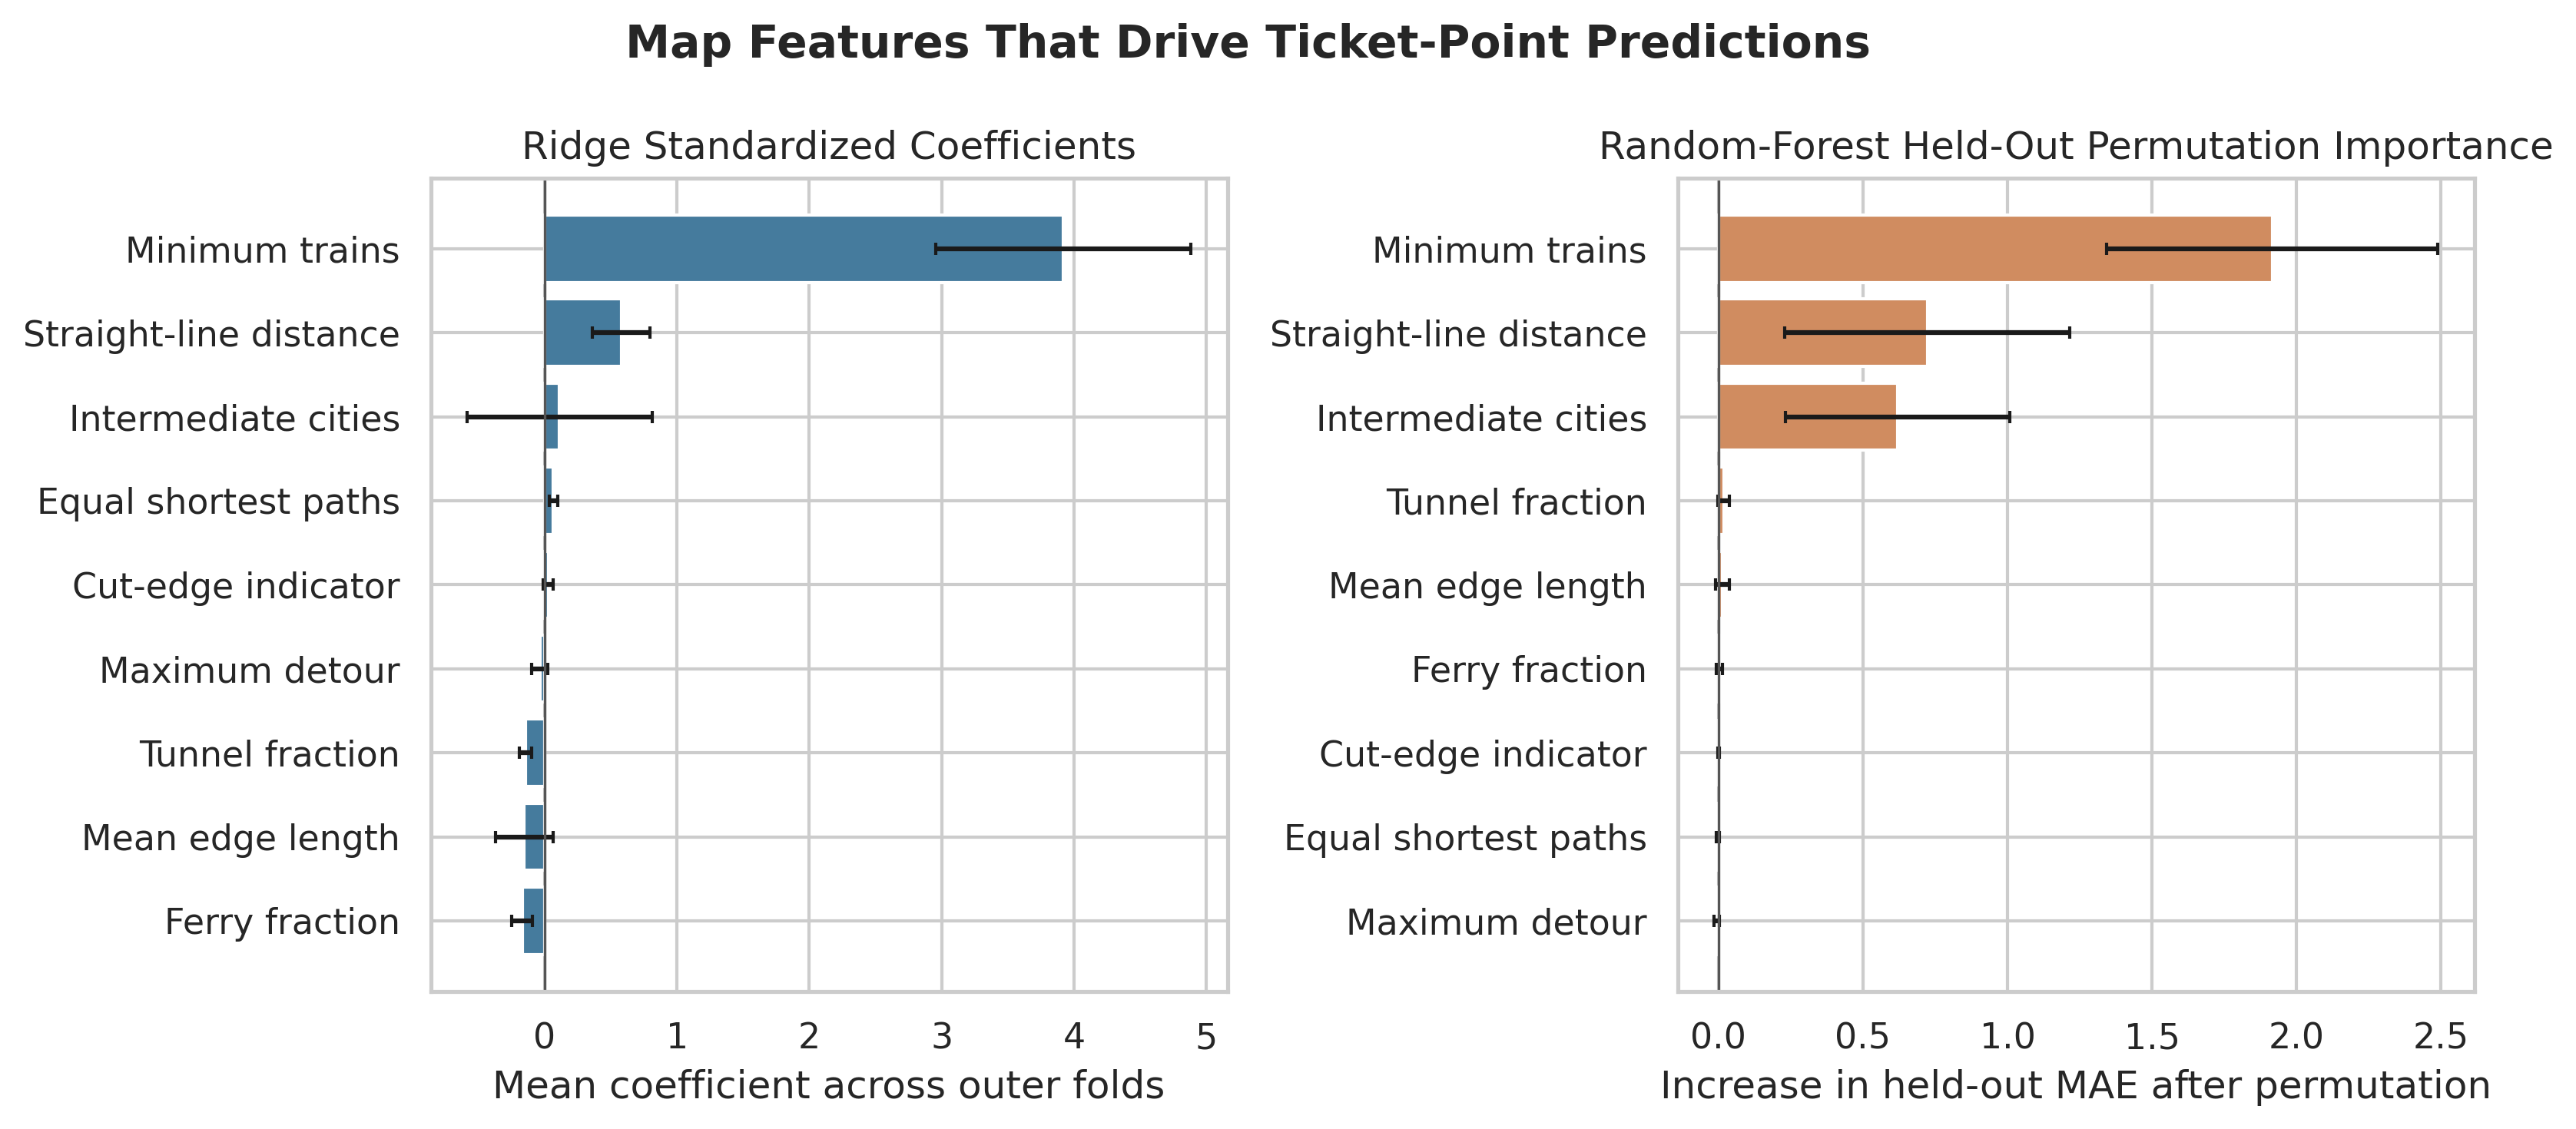
\includegraphics[width=0.80\textwidth]{../figures/feature_importance.png}
\caption{\textbf{Outer-fold feature interpretation.} Minimum trains has mean
Ridge coefficient 3.919 after standardization and raises held-out forest MAE
by 1.916 points when permuted. Error bars show fold-to-fold SD.}
\label{fig:importance}
\end{figure}

As Figure~\ref{fig:importance} confirms, minimum trains dominates both model
families. Straight-line distance and intermediate-city count carry additional
but correlated scale information. Most redundancy, tunnel, ferry, and detour
measures are near zero, sometimes slightly negative under held-out
permutation. Those values mean the fitted forest did not reliably need the
feature in these folds; they do not establish that the map property is
intrinsically unimportant.

\newpage
\section*{7. Results: RQ3 -- Matched Optimizer Comparison}

The learned revision does not meet the primary success criterion. In
Table~\ref{tab:optimizer}, both methods use a median of 44 trains and connect
7 tickets, but the learned median total falls by one point and its total
points per train falls by 0.045. Within paired trials, learned efficiency is
higher 26.4\% of the time and equal 37.2\% of the time; the mean paired change
is $-0.0308$ total points per train.

\begin{table}[h]
\centering
\caption{Medians over 250 matched 12-ticket planning pools.}
\label{tab:optimizer}
\begin{tabular}{lrrr}
\toprule
Metric & Original & Learned & Learned $-$ original \\
\midrule
Printed ticket points & 67 & 66 & $-1$ \\
Route points & 63 & 62 & $-1$ \\
Total points & 130 & 129 & $-1$ \\
Ticket points per train & 1.556 & 1.523 & $-0.032$ \\
Total points per train & 3.000 & 2.955 & $-0.045$ \\
Tickets connected & 7 & 7 & 0 \\
Trains used & 44 & 44 & 0 \\
\bottomrule
\end{tabular}
\end{table}

\begin{figure}[h]
\centering
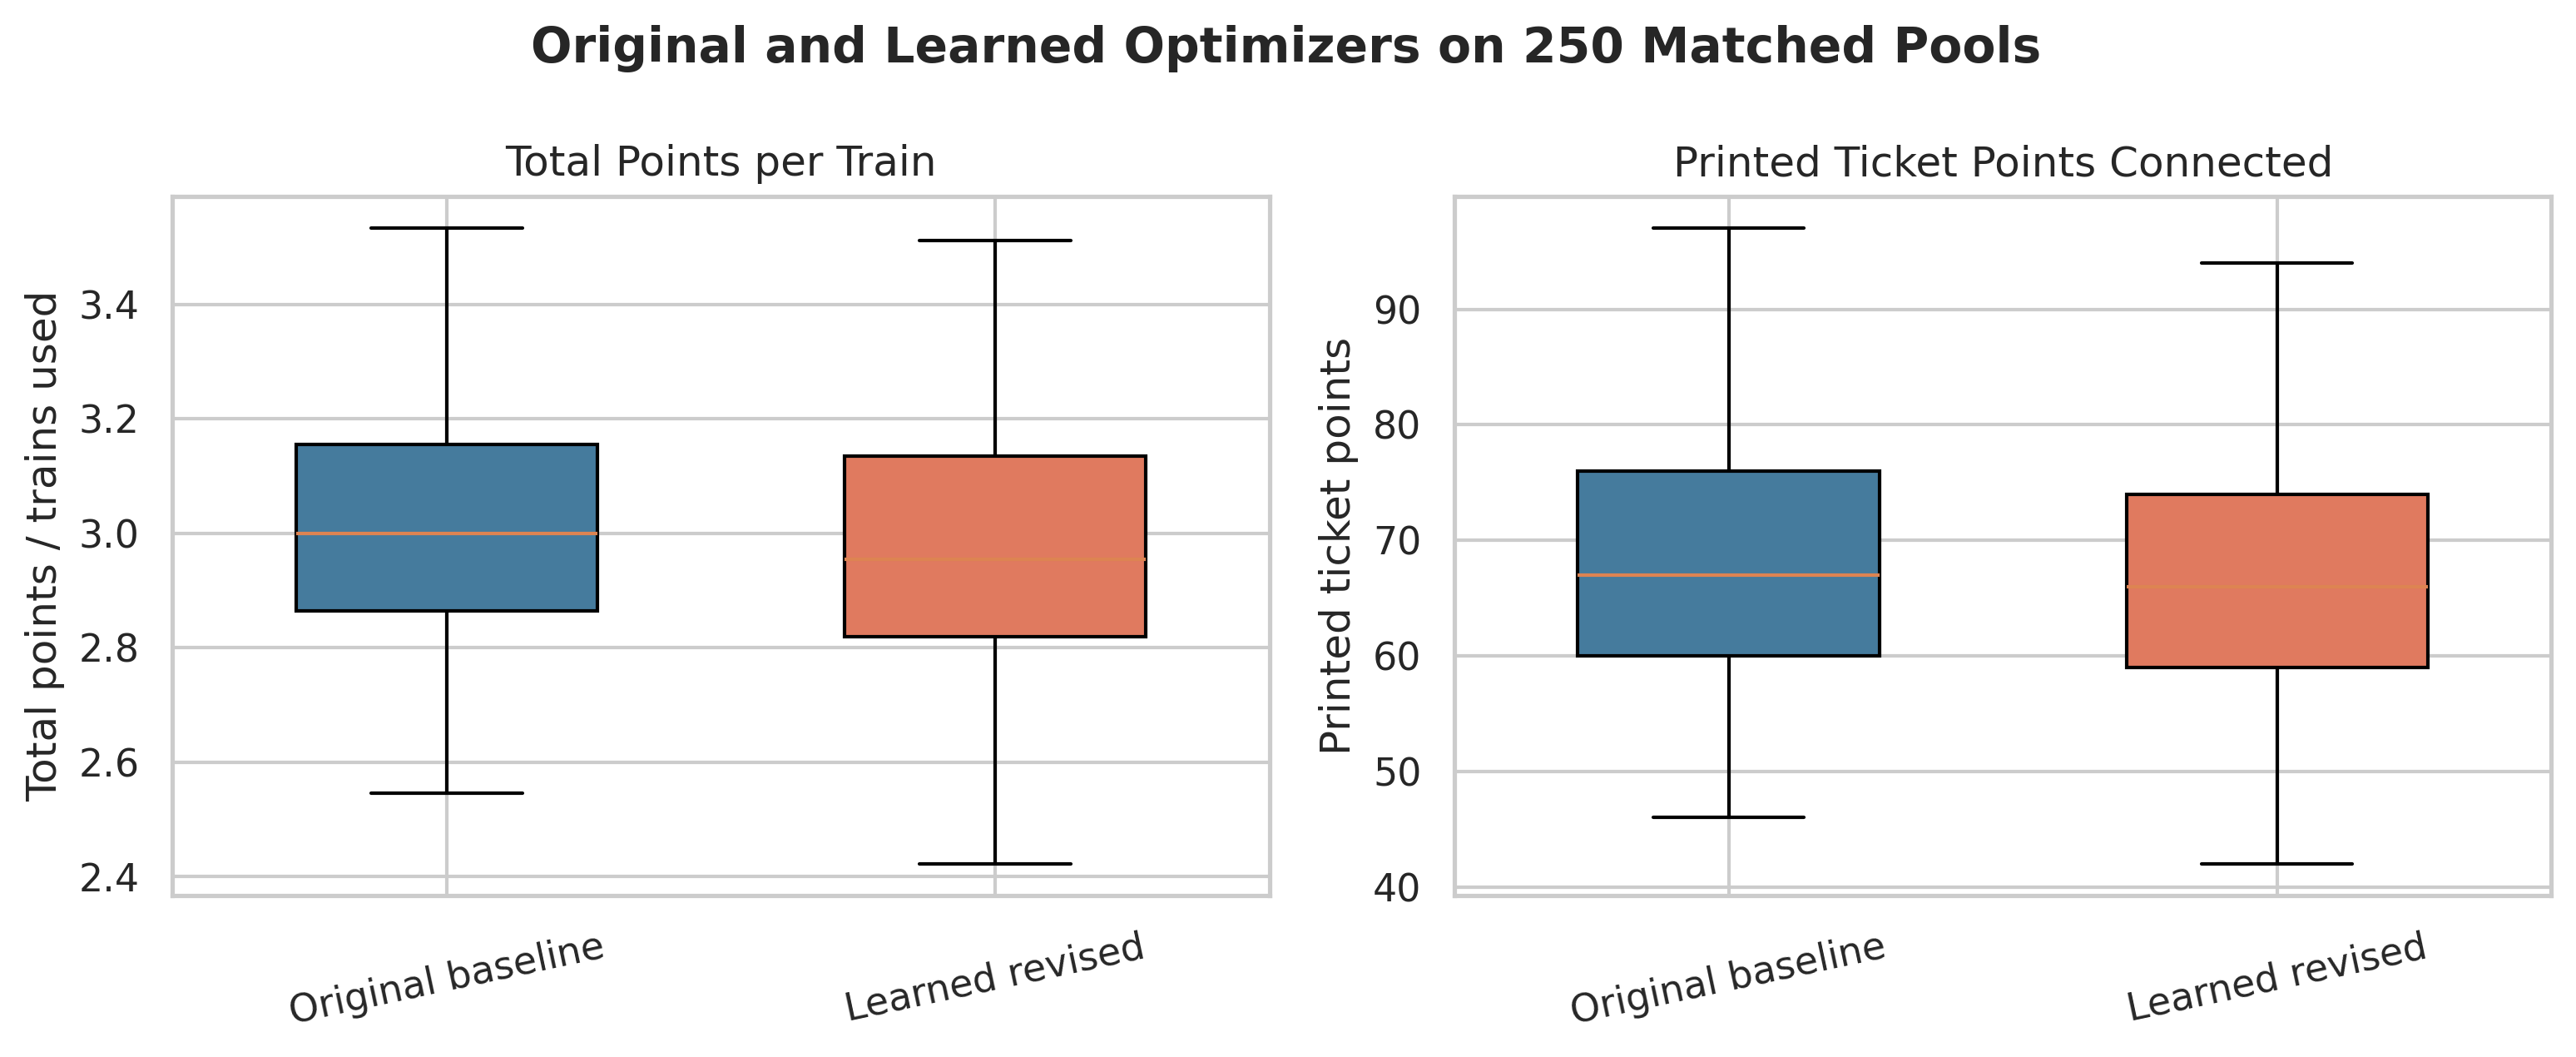
\includegraphics[width=0.82\textwidth]{../figures/optimizer_comparison.png}
\caption{\textbf{Matched optimizer outcomes.} Box plots show the central 50\%
of the same 250 pools for both methods; whiskers omit display outliers but no
trial is removed from the summaries.}
\label{fig:optimizer}
\end{figure}

\begin{center}
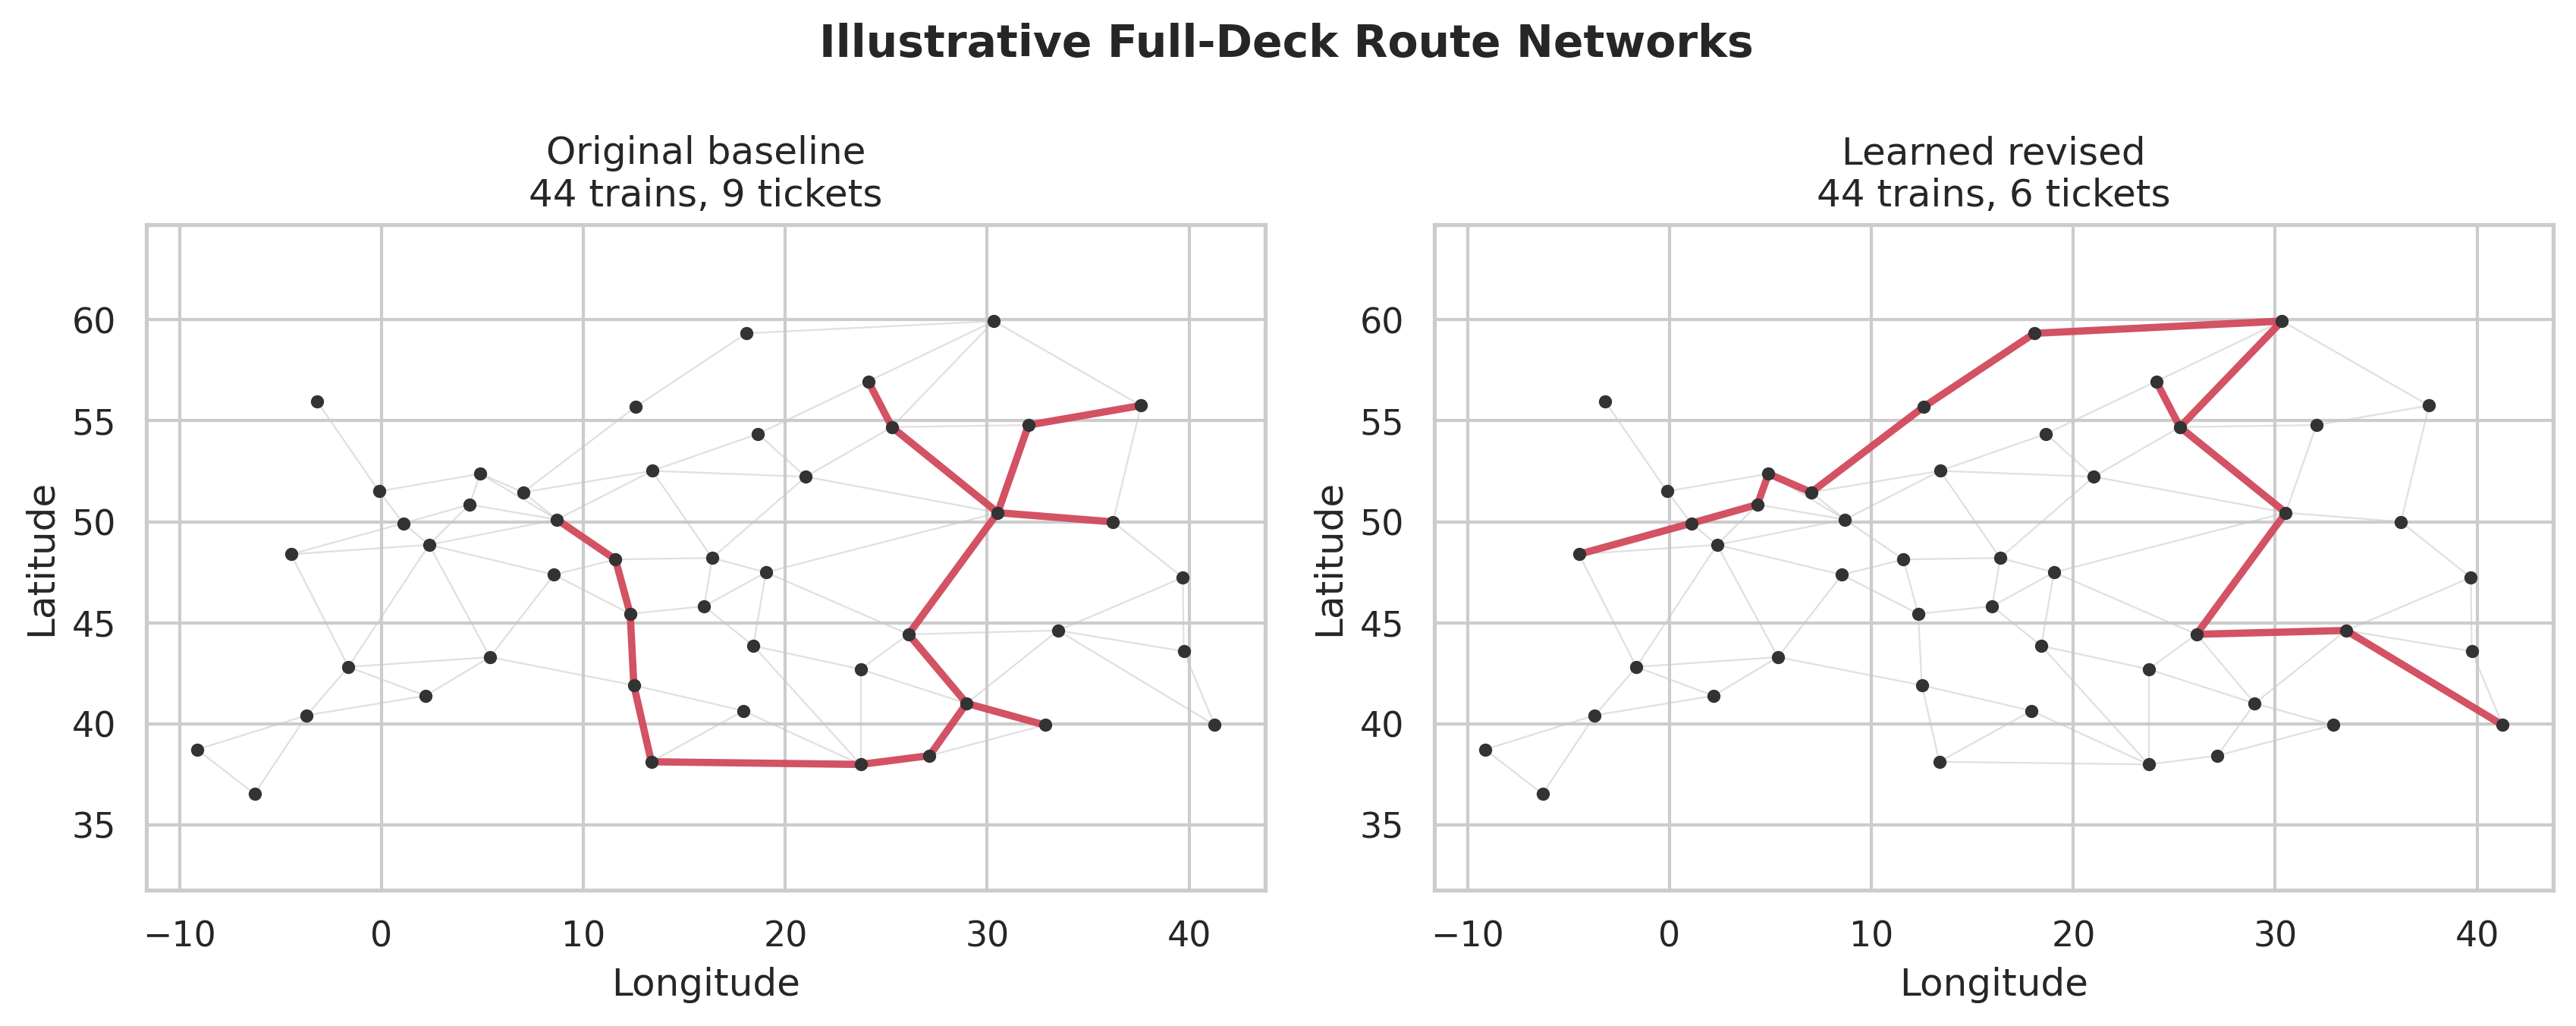
\includegraphics[width=0.60\textwidth]{../figures/selected_networks.png}
\captionsetup{hypcap=false}
\captionof{figure}{\textbf{Illustrative full-deck plans.} Red edges are selected. The
original plan scores 162 total points with 9 tickets; the revised plan scores
154 with 6. These examples visualize topology and are not substituted for the
250-pool comparison in Figure~\ref{fig:optimizer}.}
\label{fig:networks}
\end{center}

\newpage
\section*{7. Results: RQ3 -- Robustness}

Across matched pools, median mean blocked-edge retention rises from 0.9256 to
0.9284, and median worst-edge retention rises from 0.7029 to 0.7435. The mean
paired changes are only $+0.0061$ and $+0.0180$, respectively. In the
full-deck illustration, the revised network avoids all five stress edges and
retains 100\% of its 79 printed points, whereas blocking Athina--Smyrna leaves
the original plan with 21.1\% of 95 printed points. Adaptive replanning
recovers value, but the original still earns more total points in every
full-deck blocked scenario (Figure~\ref{fig:robust}).

\begin{figure}[h]
\centering
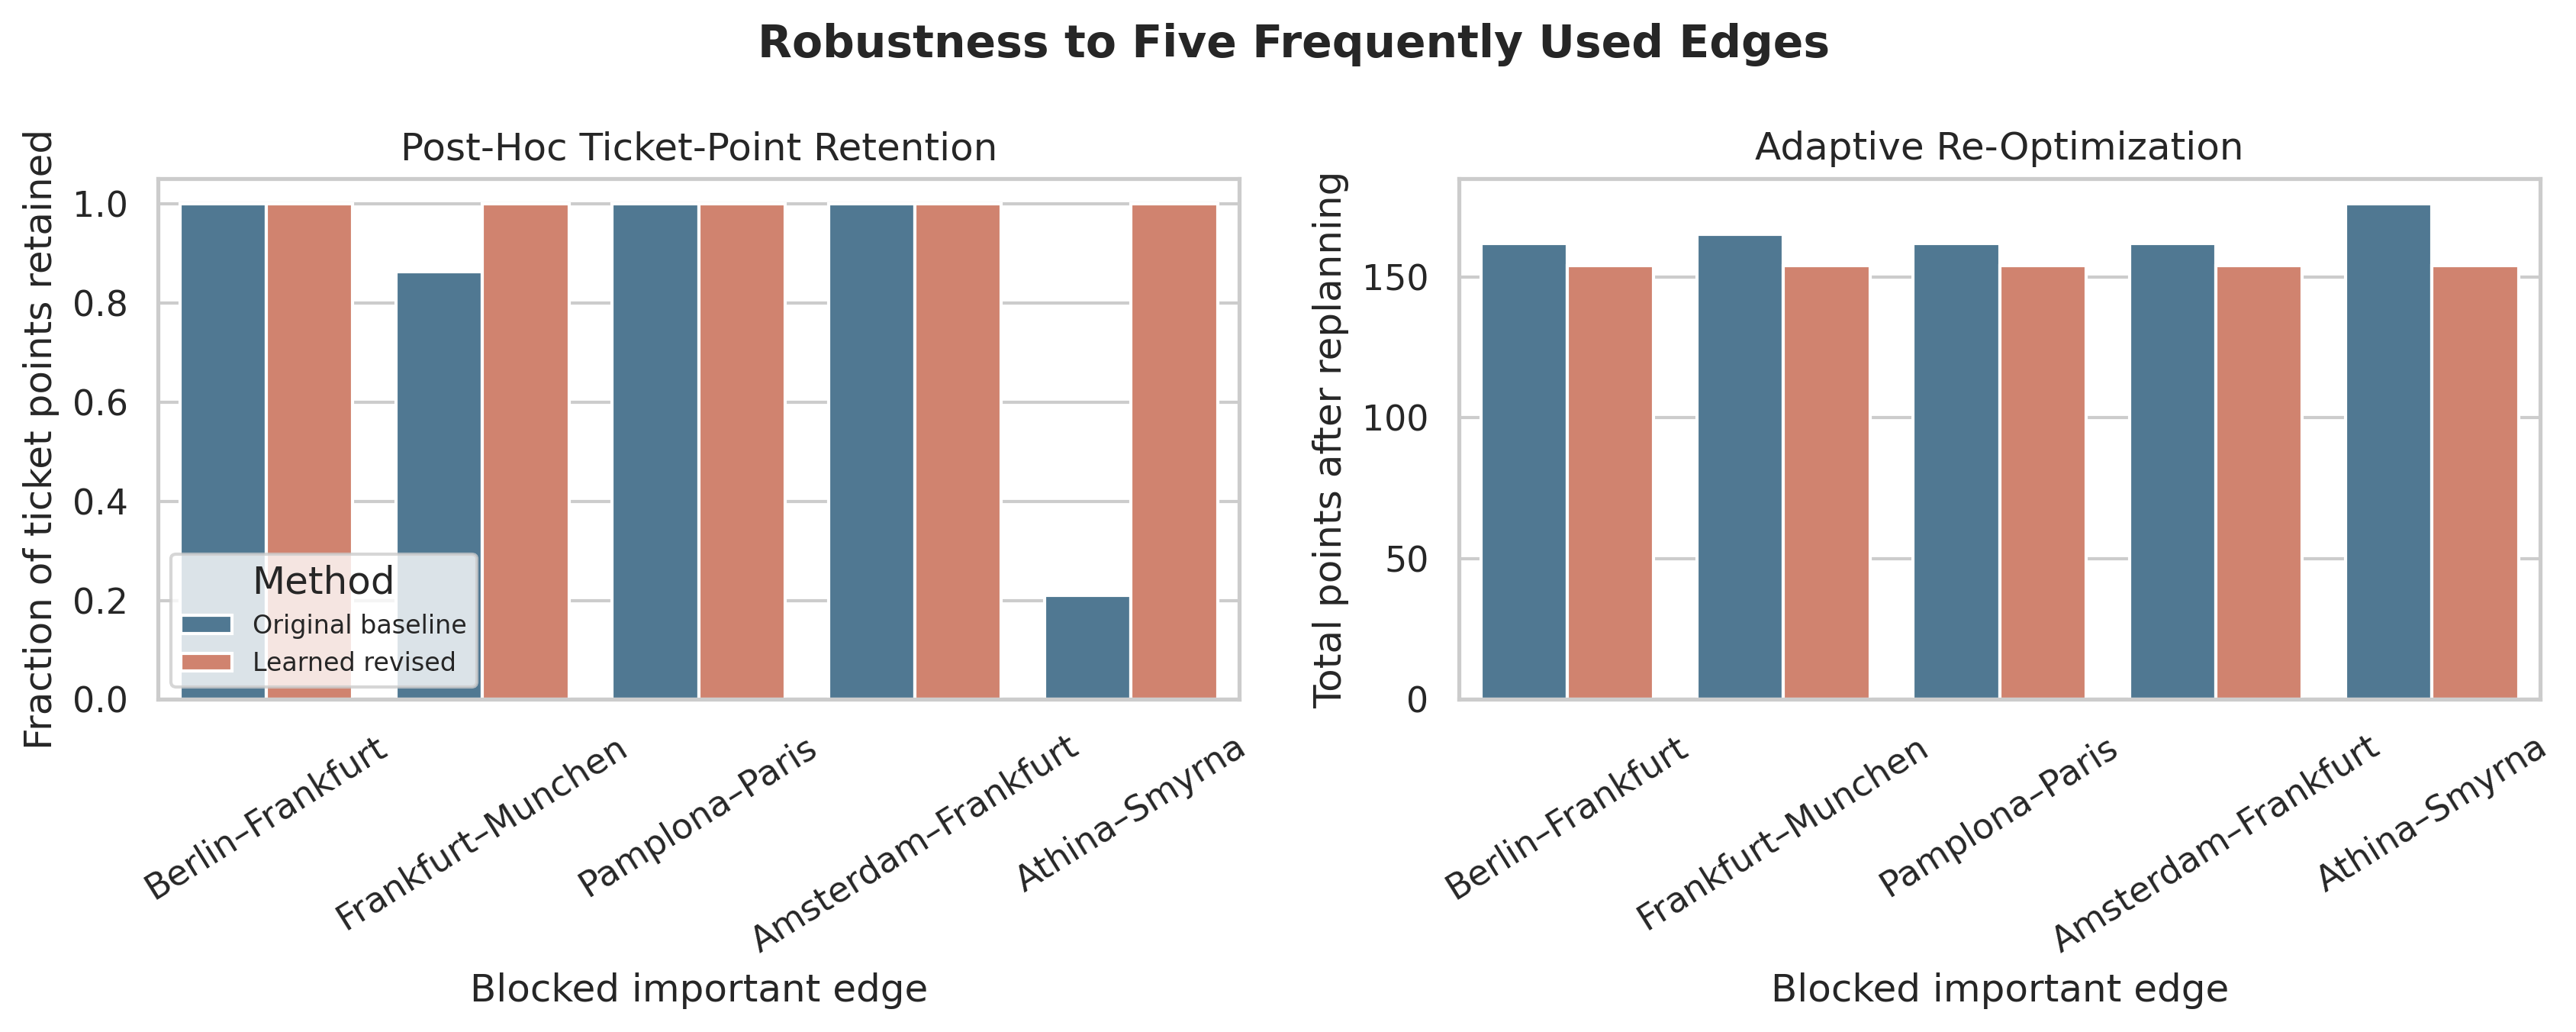
\includegraphics[width=0.91\textwidth]{../figures/optimizer_robustness.png}
\caption{\textbf{Full-deck blocked-edge stress test.} Left removes one
frequently used edge without repairs. Right reruns each method while forbidding
that edge. The revised plan is less exposed but lower scoring.}
\label{fig:robust}
\end{figure}

\section*{8. Impact and Limitations}

The analysis can help players compare visible tickets and can help students
see how graph features, leakage controls, and matched experiments interact.
Designers could also use it to audit whether ticket rewards track board cost.
It should not be presented as a gameplay guarantee. A player relying on it
could be harmed by overconfidence because the benchmark excludes opponents,
card colors, tunnel surcharges, ferry-card availability, stations, turn
timing, incomplete-ticket penalties, and the longest-route bonus.

The fan-maintained data represent one static Europe edition and only 46
tickets. The reward is nearly deterministic, predictors are correlated, and
the optimizer uses representative shortest paths and simulated accepted
pools rather than observed games. The 20\% penalty is a transparent design
choice, not an estimated causal effect. Conclusions are therefore limited to
this simplified Europe planning setting and need multiplayer simulation or
real-game validation before strategic deployment.

\newpage
\section*{9. Challenge Goals}

\textbf{Machine Learning was achieved.} The project compares three model
families on identical repeated outer folds, tunes two families only within
training data, generates OOF values, and computes held-out permutation
importance. \textbf{Multiple Datasets was achieved.} Every destination row
uses coordinates from \code{cities.csv}, graph structure from
\code{routes.csv}, and reward from \code{destinations.csv}. RQ3 then combines
that table with the route-scoring network.

\section*{10. Work Plan Evaluation}

I did not maintain a contemporaneous timer, so I avoid inventing precise
``actual hours.'' Relative to the proposal: data acquisition was faster than
the planned two hours; graph features took at least the planned five because
tie counting and edge-removal cases required testing; EDA remained close to
the planned three; nested model evaluation required more computation than the
planned five; optimizer integration required the most redesign because the
old USA representation had to be replaced by a Europe accepted-pool
benchmark; and testing/report QA exceeded the planned four. The six planned
work packages were all completed, but implementation and verification shifted
effort toward leakage control, matched evaluation, and reproducibility.

\section*{11. Testing}

\code{python test\_project.py} runs 11 named tests and ends with
``All tests passed!'' Tests cover Dijkstra cost/path/equal ties, excluded and
unreachable edges, haversine distance, validation failures, exact dataset and
Part 2 invariants, leakage exclusion, fast nested CV and complete OOF
coverage, optimizer connectivity and 45-train feasibility, identical matched
pools, deterministic seeds, and blocked-edge/adaptive behavior. The full
analysis also completed without warnings. Running \code{python -m flake8}
on all five Python modules produces no output.

\section*{12. Citations and Collaboration}

[1] L. Simon, \textit{Data \& Analysis of Ticket to Ride: Europe},
\url{https://github.com/leonsi7/ticket-to-ride-europe}, accessed August 17,
2026. [2] Days of Wonder, \textit{Ticket to Ride: Europe Rules}, 2019,
\url{https://ncdn0.daysofwonder.com/tickettoride/en/img/7202-T2RE-Rules-EN-2019.pdf}.
[3] scikit-learn, \textit{RepeatedKFold documentation},
\url{https://scikit-learn.org/stable/modules/generated/sklearn.model_selection.RepeatedKFold.html}.
[4] scikit-learn, \textit{Permutation Feature Importance},
\url{https://scikit-learn.org/stable/modules/permutation_importance.html}.
[5] CSE 163, \textit{Final Project: Report and Code},
\url{https://courses.cs.washington.edu/courses/cse163/26su/report-code/}.

I worked independently and did not consult other students. I adapted the
objective from my earlier self-authored planning heuristic. I used OpenAI
ChatGPT to assist with code organization, tests, debugging, figure/report
drafting, and specification review. I independently reran the pipeline and
checked its hand-computable cases, CSV outputs, figures, and final PDF.

\end{document}
